The H\'enon map is a two-dimensional system given by
\begin{equation}{\label{eq:hem}}
	\begin{aligned}
		x_{n+1}&=y_n+1-Ax^2_n\\
		y_{n+1}&=Bx_n
	\end{aligned}
\end{equation}
Depending on the values for the parameters $A$ and $B$, iterations of (\ref{eq:hem}) lead to fixed points, periodic orbits or chaotic structures, and for $|B|>1$ the map diverges to infinity.\\
The Fixed points are given by
\begin{equation}
	\tilde{x}=\frac{(B-1)\pm\sqrt{(1-B)^2+4A}}{2A}\quad\tilde{y}=B\left(\frac{(B-1)\pm\sqrt{(1-B)^2+4A}}{2A}\right)
\end{equation}
The fixed point can be transformed to the origin and the nonlinear terms can be discarded after taking a Taylor series expansion.
\begin{equation}
	\text{For}\quad
	\begin{aligned}
		x_{n+1}&=f(x_n,y_n)\\
		y_{n+1}&=g(x_n,y_n)
	\end{aligned}\quad\rightarrow\quad
	J(\tilde{x},\tilde{y})=
	\at{
	\begin{pmatrix}
		\dfrac{\partial f}{\partial x}&\dfrac{\partial f}{\partial y}\\[10pt]
		\dfrac{\partial g}{\partial x}&\dfrac{\partial g}{\partial y}
	\end{pmatrix}}
	{x=\tilde{x},y=\tilde{y}}\quad
	J_H=
	\begin{pmatrix}
		-2A\tilde{x}&1\\
		B&0
	\end{pmatrix}
\end{equation}
The H\'enon attractor is found for the parameters $A=1.4$ and $B=0.3$.
It has the form of a horse shoe as shown in Figure (\ref{fig:hmbu})(top).
The self-similarity of this structure in the xy-plane is evident from multiple blowups of the regions inside the squares in Figure (\ref{fig:hmbu})(bottom).
If one of the parameter is kept at a fixed value and the other is varied, bifurcation diagrams can be calculated as shown in Figure (\ref{fig:hmbf}).\\
\begin{figure}[h!]
	\centering
	\begin{subfigure}{0.45\linewidth}
		\centering
		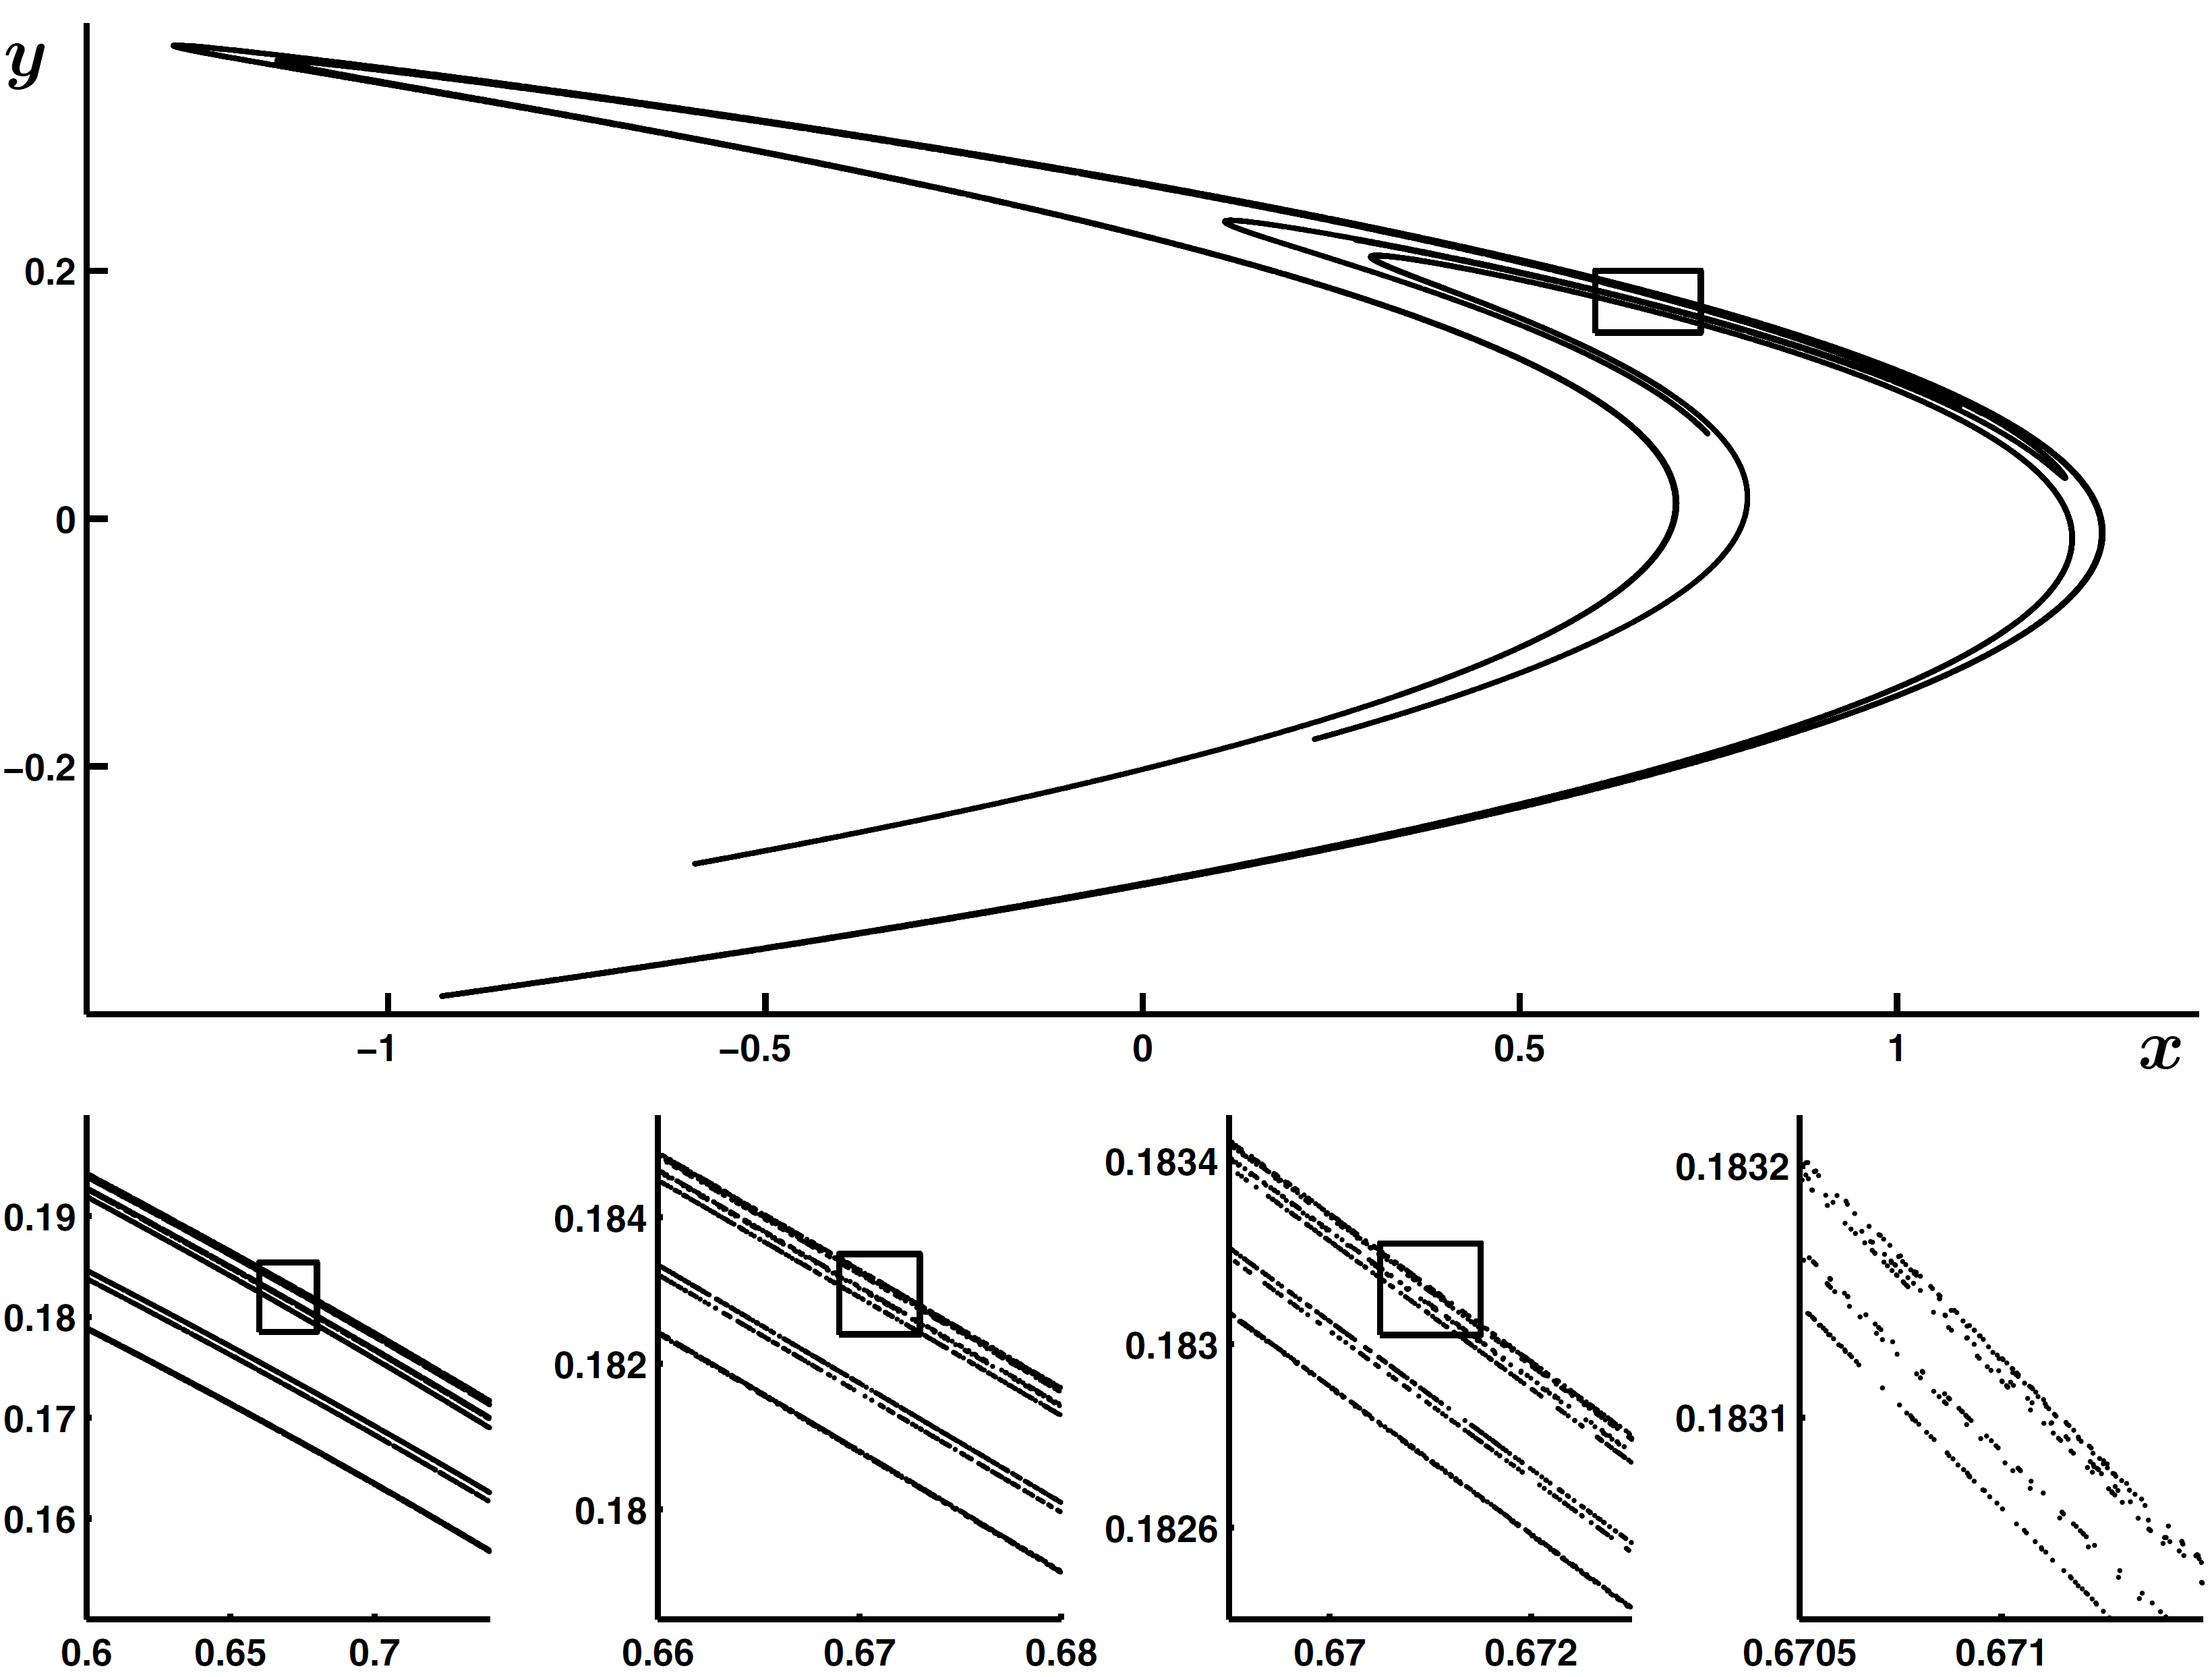
\includegraphics[width=\linewidth]{hmbu.png}
		\caption{The H\'enon attractor (top) and blowups (bottom) demonstrating the finestructure and self-similarity of the attractor in the $xy$-plane.}
		\label{fig:hmbu}
	\end{subfigure}
	\vline
	\begin{subfigure}{0.5\linewidth}
		\centering
		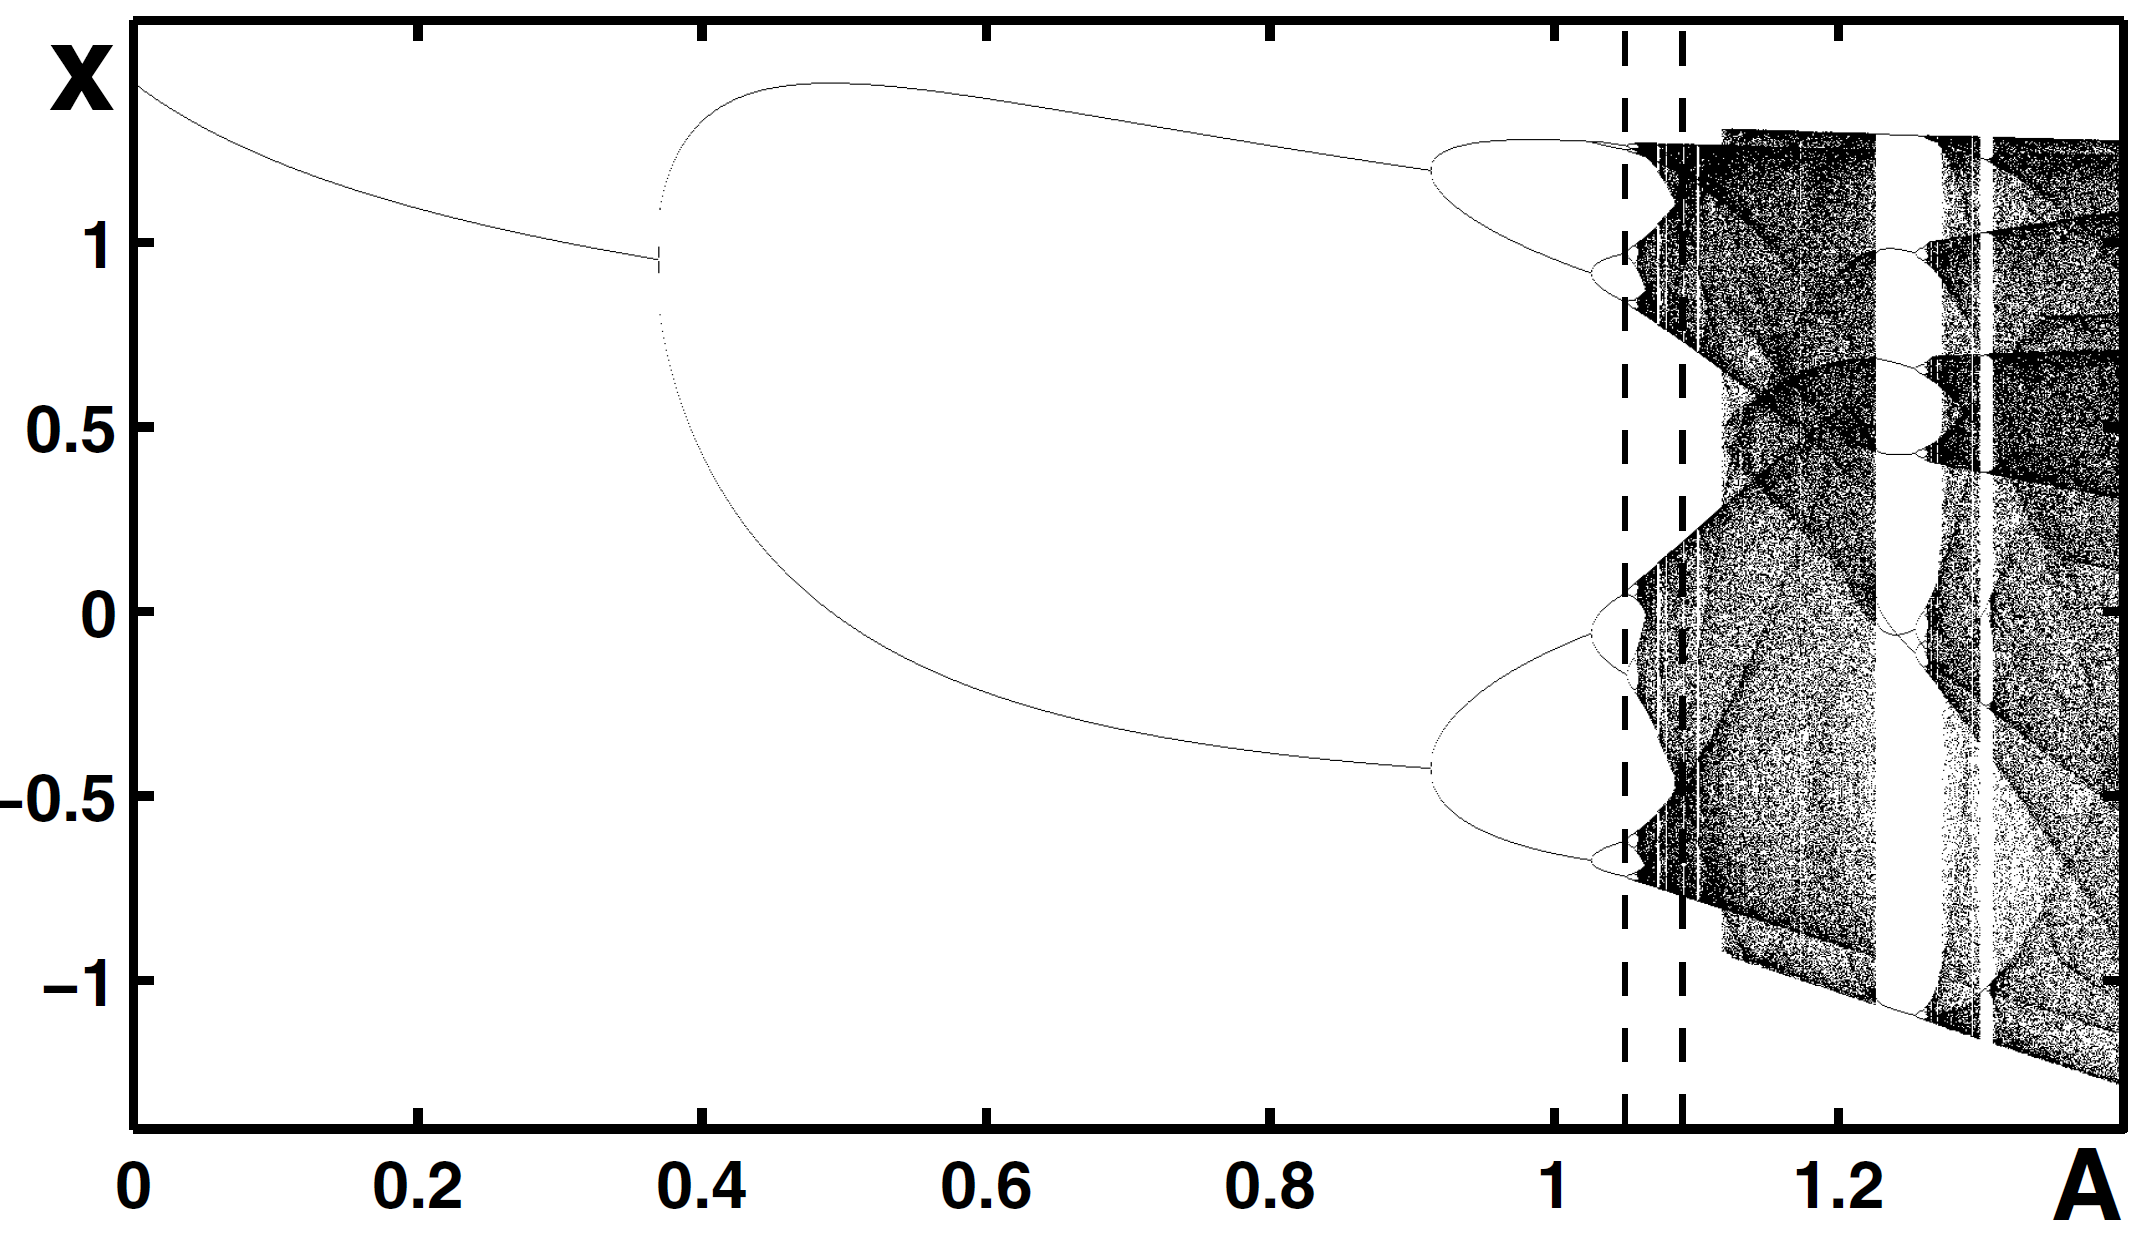
\includegraphics[width=\linewidth]{hmbf.png}
		\caption{Bifurcation diagram for the H\'enon map.\\Stationary, periodic and chaotic orbits for $x$ with $B=0.3$ and $0\leq A\leq1.4$.\\The map shows bistability and hysteresis.}
		\label{fig:hmbf}
	\end{subfigure}
	\caption{}
\end{figure}
An interesting region in parameter space exists in the H\'enon map for $B=0.3$ and $1.147022\leq A\leq1.1470615$ (Figure (\ref{fig:hmfsbu})).
\begin{figure}[h!]
	\centering
	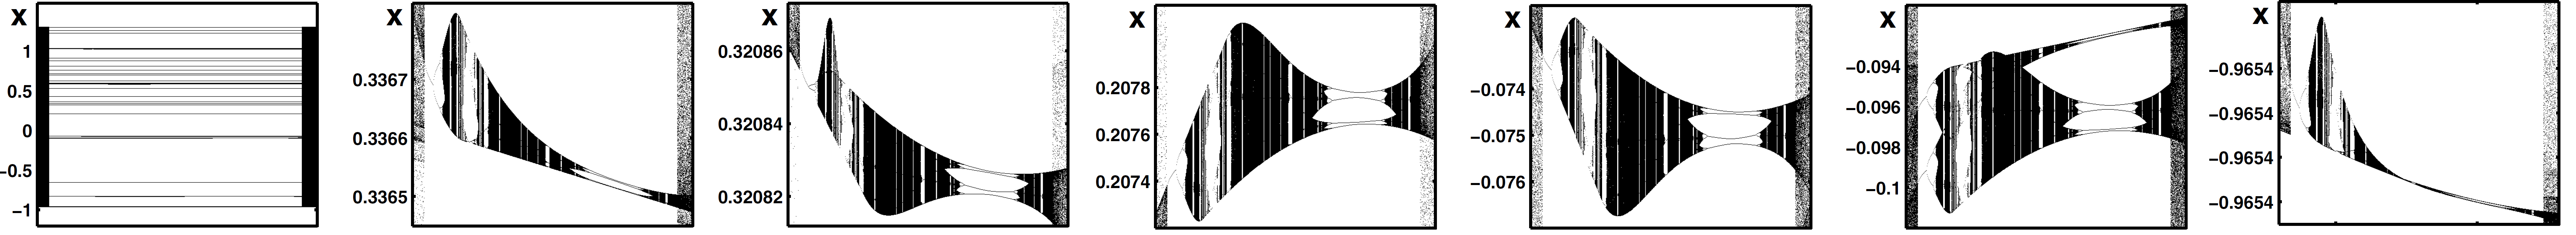
\includegraphics[width=1.1\linewidth]{hmfsbu.png}
	\caption{Blowups demonstrating the fine-structure in the bifurcation diagram of the H\'enon map in the directions of the variable $x$ and the parameter $A$.}
	\label{fig:hmfsbu}
\end{figure}